\subsection{Resonant Path, Transformer, and Rectifier}
\label{sec:hw-output}

The transformer primary is connected to VSW through the resonant capacitor and added series inductance. CR1--CR4 rectify the secondary energy into a bulk supply for the MPQ4242 output stage. The USB-C PD stage regulates the output voltage from this bulk supply.

Several inductor arrangements were tried during bring-up. The final assembly has two Wurth Elektronik 7443640470B inductors connected in series, each nominally \SI{4.7}{\micro\henry}. Together they add \SI{9.4}{\micro\henry}, with an individual tolerance of \(\pm20\%\). Each has a maximum DC resistance of \SI{0.97}{\milli\ohm} at \SI{20}{\celsius}, giving \SI{1.94}{\milli\ohm} for the pair before the connecting wires \cite{wurth7443640470b}. Both parts carry the same current. Loss is spread across the two packages, but either part's temperature can still limit operation.

With approximately \SI{16.5}{\micro\henry} transformer leakage and the \SI{1}{\nano\farad} capacitor, the first-order resonance lies near the \SI{1}{\mega\hertz} carrier. That estimate depends on the fitted transformer, component tolerances, and connecting conductors, as explained in \cref{sec:analysis-resonant,sec:mag-parasitics}. The L4 value in V1.1 does not represent this final series pair.

\begin{figure}[H]
\centering
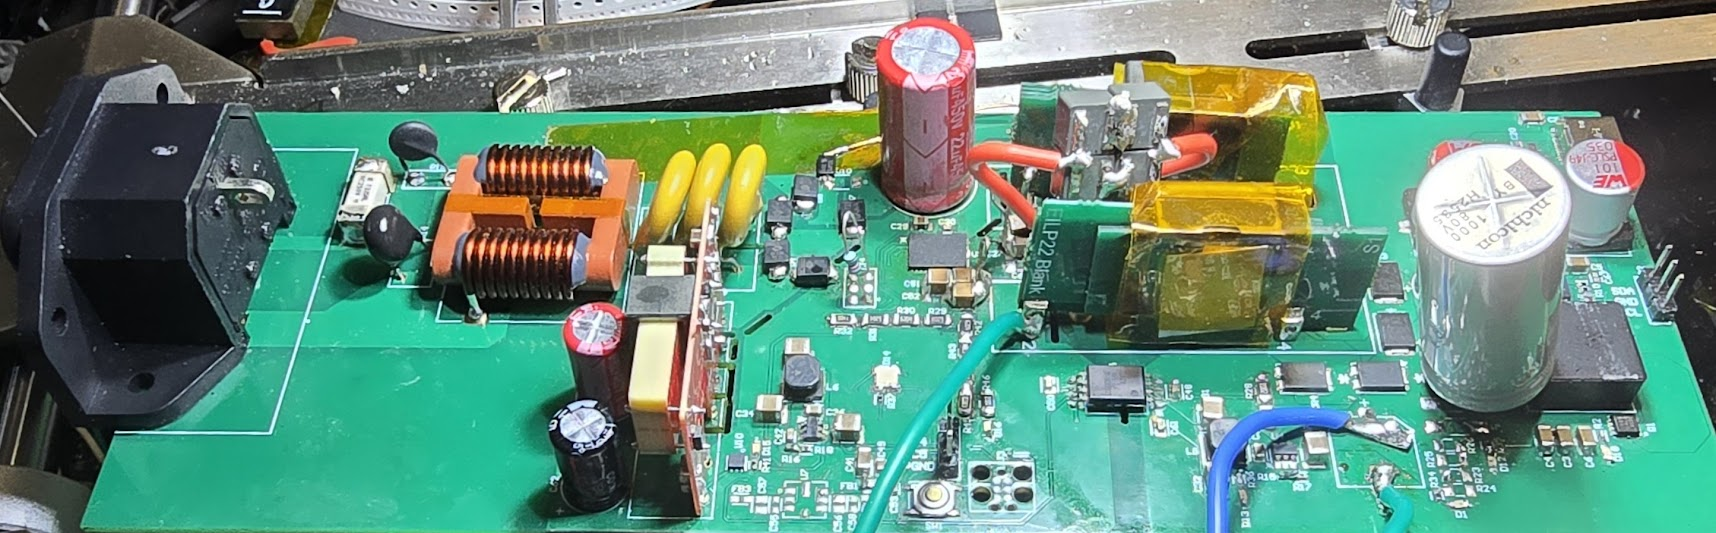
\includegraphics[width=\textwidth,height=0.35\textheight,keepaspectratio]{Pictures/Thesis/07_Hardware/resonant_inductor_test_variants.png}
\caption{Resonant-inductor arrangements tested during bring-up.}
\label{fig:resonant-inductor-test-variants}
\end{figure}

\begin{figure}[H]
\centering
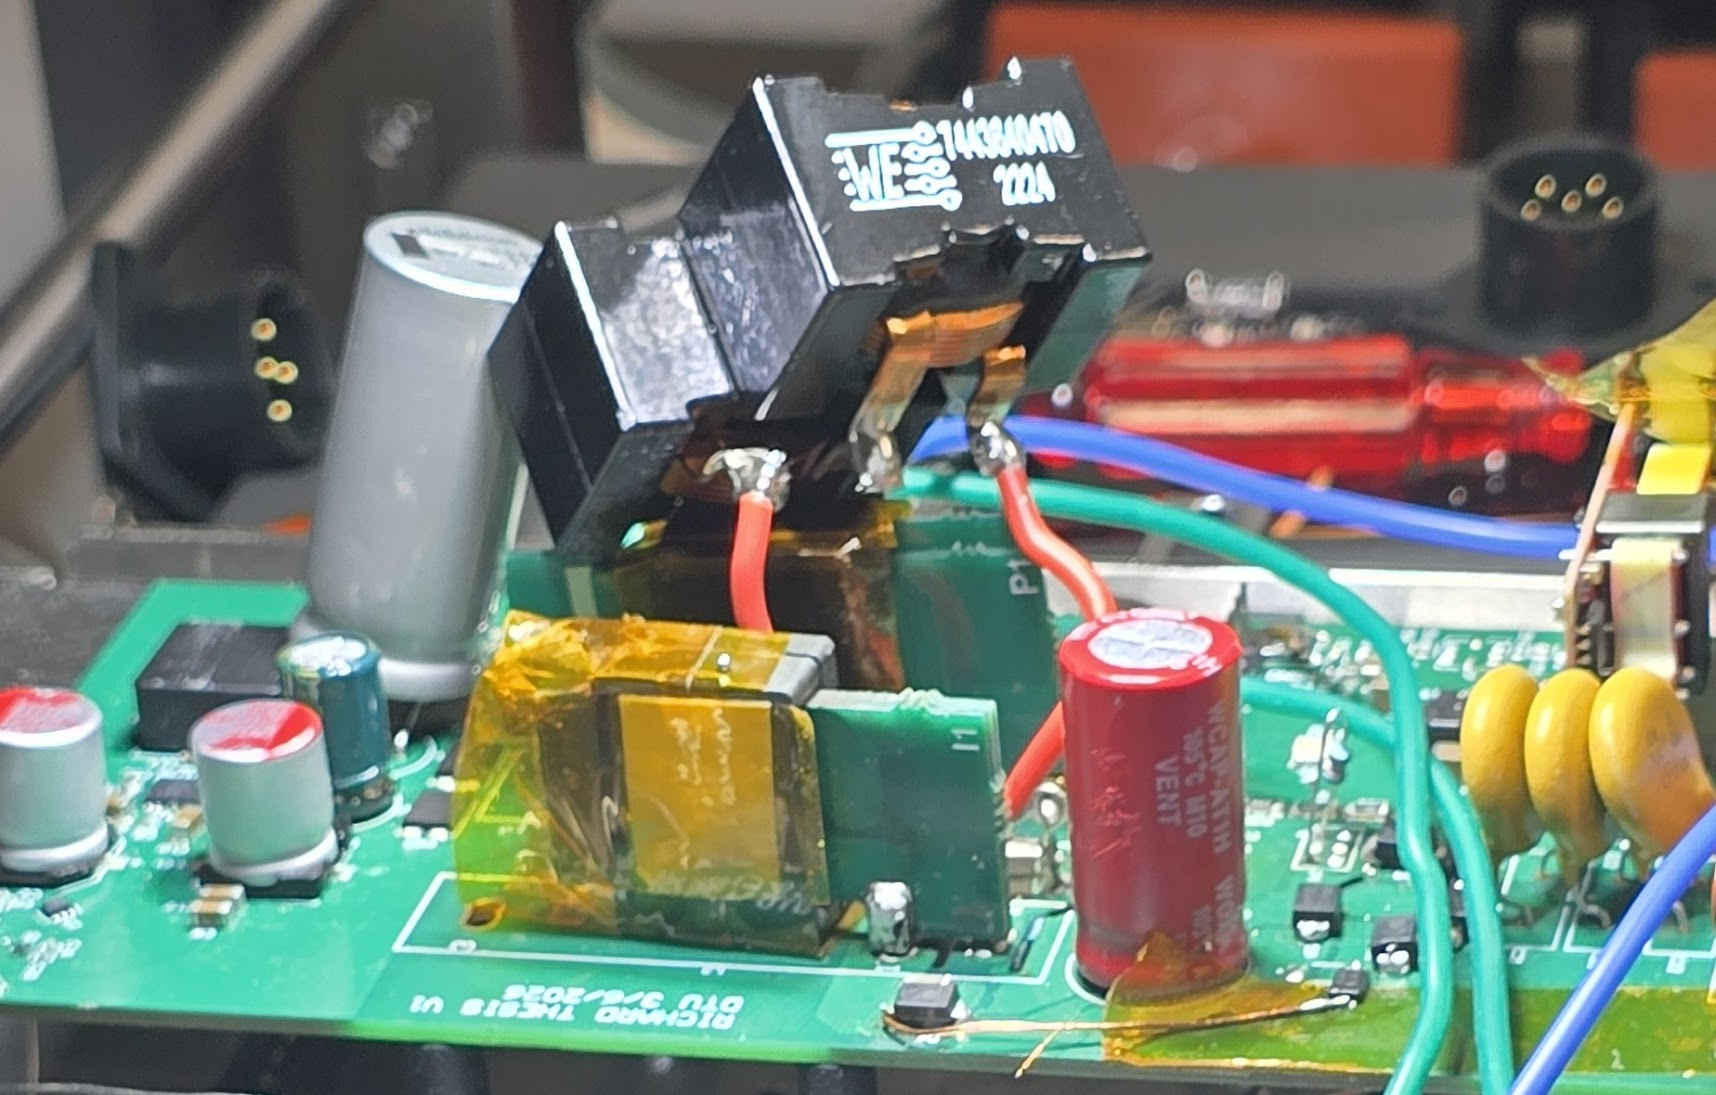
\includegraphics[width=\textwidth,height=0.35\textheight,keepaspectratio]{Pictures/Thesis/07_Hardware/final_resonant_inductor_usb_pdo.png}
\caption{Final series-inductor configuration and output-test arrangement.}
\label{fig:final-resonant-inductor-usb-pdo}
\end{figure}

Changing the resonant branch affects tank current, gain, and the charge available to change VSW during commutation. Waveform comparisons therefore need the fitted inductor arrangement. The installed path must be measured before the model is used to select another change.
